\section{Mohrsche Spannungskreis}
%	\vspace*{3cm}
%\textbf{Vorzeichenkonvention} \\

\begin{minipage}{0.252\linewidth}
	\begin{align*}
		\tau	 		&= \gamma \cdot sin(\beta) \cdot cos(\beta) \\
		\sigma_{h=x} 	&= \sigma_v \cdot K_0 \\
		\sigma_{v=y} 	&= \gamma \cdot h \cdot cos(\beta)^2 \\ 
	\end{align*}
\end{minipage}
\begin{minipage}{0.5\linewidth}
	\begin{align*}
		\sigma_{max=1}	&=\frac{1}{2} \cdot (\sigma_x + \sigma_y) + \sqrt{\left(\frac{\sigma_y - \sigma_x}{2}\right)^2 + \tau_{xy}^2} \\
	\sigma_{min=3}	&=\frac{1}{2} \cdot (\sigma_x + \sigma_y) - \sqrt{\left(\frac{\sigma_y - \sigma_x}{2}\right)^2 + \tau_{xy}^2} \\
	\end{align*}
\end{minipage}
\begin{minipage}{0.5\linewidth}
	\begin{align*}
	MP				&= \frac{\sigma_1 + \sigma_3}{2} \\
	r				&= MP - \sigma_3 \\
	\end{align*}
\end{minipage}



%\begin{minipage}[t]{0.1\linewidth}
%	\begin{align*}
%		\tau	 		&= \gamma \cdot sin(\beta) \cdot cos(\beta) \\
%		\sigma_{h=x} 	&= \sigma_v \cdot K_0 \\
%		\sigma_{v=y} 	&= \gamma \cdot h \cdot cos(\beta)^2 \\ 
%		\sigma_{max=1}	&=\frac{1}{2} \cdot (\sigma_x + \sigma_y) + \sqrt{\left(\frac{\sigma_y - \sigma_x}{2}\right)^2 + \tau_{xy}^2} \\
%		\sigma_{min=3}	&=\frac{1}{2} \cdot (\sigma_x + \sigma_y) - \sqrt{\left(\frac{\sigma_y - \sigma_x}{2}\right)^2 + \tau_{xy}^2} \\
%	 \\
%		MP				&= \frac{\sigma_1 + \sigma_3}{2} \\
%		r				&= MP - \sigma_3 \\
%	\end{align*}
%\end{minipage}	
%\textbf{Mohrsche Kreis Bsp/Visualisierung} \\


\begin{minipage}{0.7\linewidth}
	\begin{align*}
		\sigma_\alpha	&=\sigma_{max=1} \cdot cos(\alpha)^2 + \sigma_{min=3} \cdot sin(\alpha)^2 \\
		\tau_\alpha		&= (\sigma_{max} -\sigma_{min}) \cdot cos(\alpha) \cdot sin(\alpha) \\
		\sigma_n		&= \sigma_x \cdot cos(\alpha)^2 + \sigma_y \cdot sin(\alpha)^2 + 2 \cdot \tau_{xy} \cdot cos(\alpha) \cdot sin(\alpha) \\
		\sigma_t		&= \sigma_x \cdot cos(\alpha)^2 + \sigma_y \cdot sin(\alpha)^2 - 2 \cdot \tau_{xy} \cdot cos(\alpha) \cdot sin(\alpha) \\
		\tau_?			&= \tau_{xy} (cos(\alpha)^2 - sin(\alpha)^2) - \sigma_x \cdot cos(\alpha) \cdot sin(\alpha) + \sigma_y \cdot cos(\alpha) \cdot sin(\alpha)
	\end{align*}
\end{minipage}
\begin{minipage}{0.5\linewidth}
	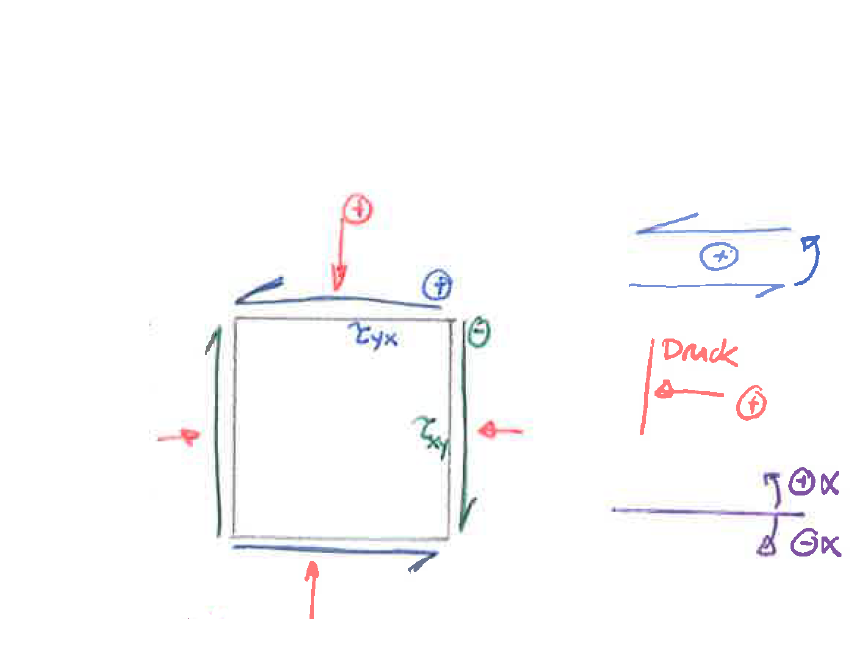
\includegraphics[width=0.5\linewidth]{images/Mohrsch1Vorzeichen.PNG} \\
	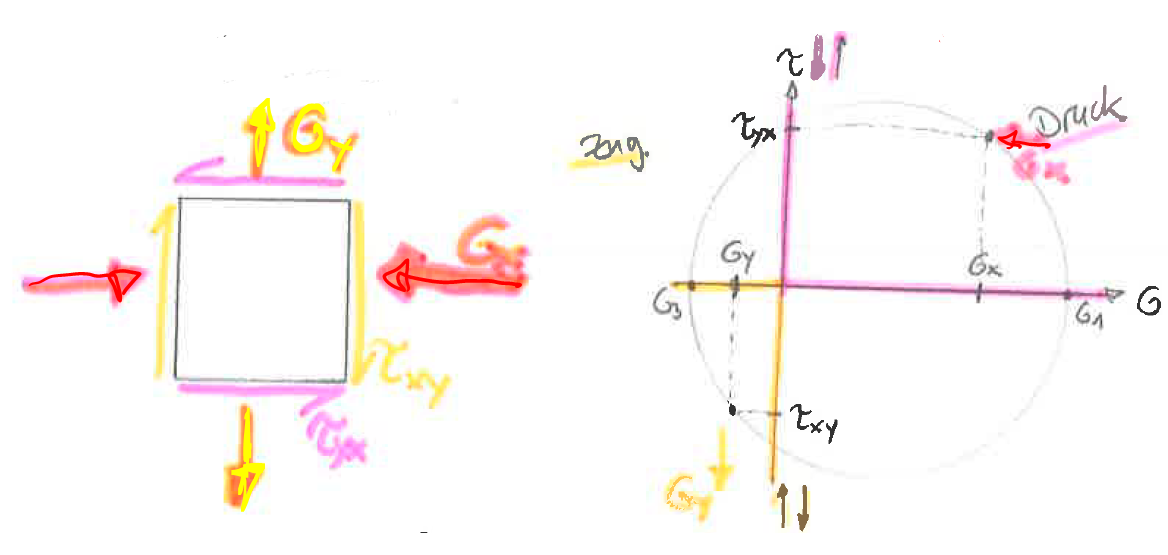
\includegraphics[width=0.65\linewidth]{images/Mohrsch2Bsp.PNG}
\end{minipage}

%\textbf{Pol Visualisierung}
%	\vspace*{4cm}
\begin{minipage}{0.45\linewidth}
	\bigskip
	\begin{align*}
		tan(2 \alpha)	&= \frac{2 \tau}{\sigma_y - \sigma_x} \\
		\tau_{max}		&= tan(2 \alpha) = \frac{\sigma_y - \sigma_x}{2} \cdot sin(2 \alpha) \\
		\rightarrow \alpha &= 45° \Rightarrow \tau_{max} \\ 
	\end{align*}
\end{minipage}
\begin{minipage}{0.5\linewidth}
	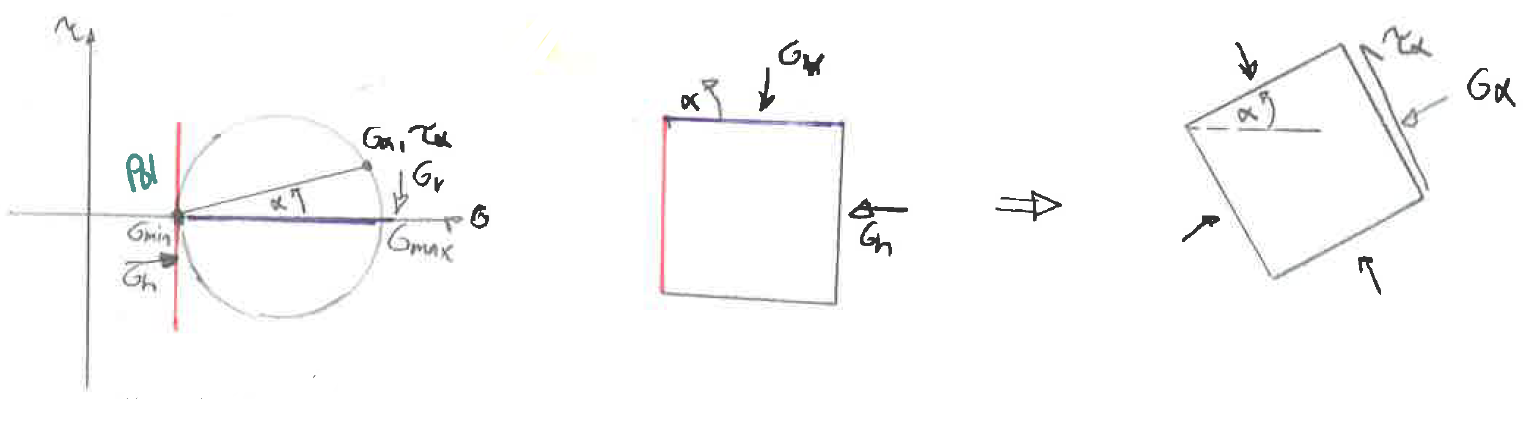
\includegraphics[width=\linewidth]{images/Mohrsch3BspPol.PNG}
\end{minipage}